\section{Auswertung}
\subsection{Kalibrierkurve}
Bevor der eigentlichen Messung der Hysteresekurven, soll die Kalibirerkurve für das Magnetfeld gemessen werden. Dazu mittels einer Hall-Sonde das Magnetfeld gemessen. Die gemessenen Daten sind in der Abbildung \ref{fig:Kalibrierung} dargestellt. Die gemessene Kalibrierkurve ist nicht linear, wie sie es aber im Idealfall sein sollte. Die Ursache für die Nichtlinearität ist die Sättigung des Eisenkerns. 
\begin{figure}[H]
\centering
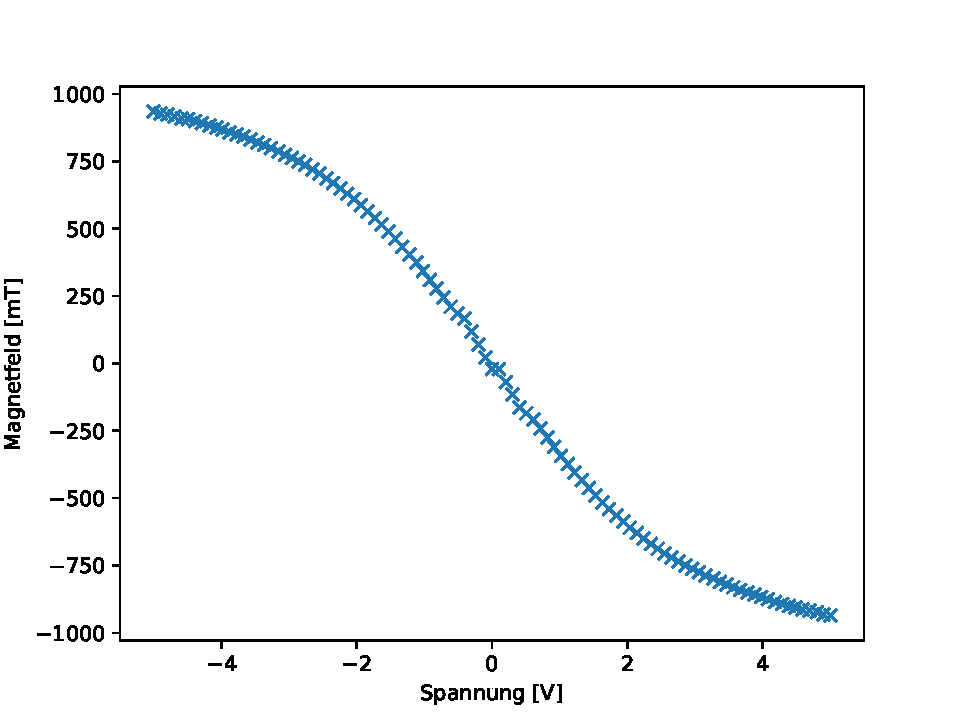
\includegraphics[scale=0.8]{../Messdaten/auswertung/Kalibrierung.pdf}
\caption{ Das Magnetfeld für unterschiedliche Spannungen der Position der Probe innerhalb der Spule. Zu sehen ist eine nichtlinearer Zusammenhang der Kalibrierungskurve. }
\label{fig:Kalibrierung}
\end{figure}


\subsection{Temperaturabhängigkeit der Hysteresekurven}
Für die Berechnunug des Kerr-Winkels wird der Zusammenhang zwischen der Drehung der Mikrometerschraube mit der gemessenen Spannung benötigt. Die gemessenen Werte sind in der Tabelle \ref{tab:Mikrometerschraube} dargestellt. Aus der Stellung der Mikrometerschraube kann der Winkel berechnet werden, wobei gilt $ 1 \mathrm{Tick}\ \widehat{=}\ 0.024\ {}^\circ$. Gut erkennbar ist der erwartete lineare Zusammenhang zwischen Kerr-Winkel und Spannung.
\begin{table}[h]
    \centering
    \caption{
        Zusammenhang zwischen Stellung der Mikrometerschraube des Polarisationsfilters und  des Kerr-Winkels mit der Spannung.
        }
    \label{tab:Mikrometerschraube}
    \begin{tabular}{r|c|l}
    Mikrometerschraube [ticks] & Kerr-Winkel [${}^\circ$]& Spannung [V] \\\hline
    0  & 0 & 0
 \\
    10 & 0.24 & 0.1
 \\
    20 & 0.48 & 0.2
 \\
    30 & 0.72 & 0.3
 \\
    40 & 0.96 & 0.4
 \\
    50 & 1.2 & 0.5 \\   
    \end{tabular}
\end{table}
Die unbearbeitete Hysteresekurve in der Abbildung \ref{fig:hysterese_original} ist schräg und nicht gerade. Die Ursache dafür ist, dass in der Polymerschicht die sich auf der magnetooptischen Disk befindet es auch zu einer Polarisationsänderung kommt. Diese Polarisationsänderung gibt es zusätzlich zu der Polarisationsänderung durch den Kerr-Effekt. Zur Bestimmung der Kerr-Winkel muss somit der Einfluss der Polymerschicht rausgerechnet werden.  
\begin{figure}[H]
\centering
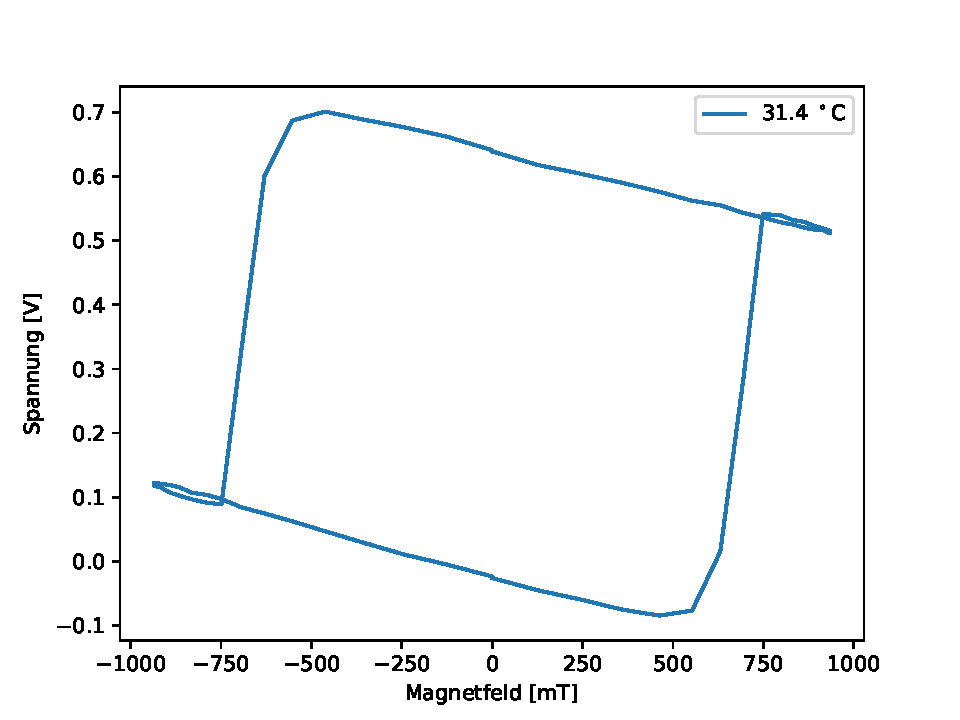
\includegraphics[scale=0.8]{../Messdaten/auswertung/hysterese_7_original.pdf}
\caption{ Unbearbeitete Hysteresekurve bei einer Temperatur von $31,4\ {}^\circ$C.}
\label{fig:hysterese_original}
\end{figure}


\begin{figure}[H]
\centering
    \subfig{../Messdaten/auswertung/hysterese_7.pdf}
    \subfig{../Messdaten/auswertung/hysterese_8.pdf}
    \subfig{../Messdaten/auswertung/hysterese_9.pdf}
    \subfig{../Messdaten/auswertung/hysterese_10.pdf}
    \subfig{../Messdaten/auswertung/hysterese_11.pdf}
    \subfig{../Messdaten/auswertung/hysterese_12.pdf}
    
    
    
\caption{ Hysteresekurven für unterschiedliche Temperaturen.  }
\label{fig:hysterese_temp_1}
\end{figure}

\begin{figure}[H]
\centering
\subfig{../Messdaten/auswertung/hysterese_13.pdf}
    \subfig{../Messdaten/auswertung/hysterese_14.pdf}
    \subfig{../Messdaten/auswertung/hysterese_15.pdf}
    \subfig{../Messdaten/auswertung/hysterese_16.pdf}
    \subfig{../Messdaten/auswertung/hysterese_17.pdf}
\caption{ Hysteresekurven für unterschiedliche Temperaturen. }
\label{fig:hysterese_temp_2}
\end{figure}
